\documentclass[11pt,a4paper]{article}

\usepackage[T1]{fontenc}
\usepackage[utf8]{inputenc}
\usepackage{lmodern}
\usepackage[magyar]{babel}
\usepackage{newunicodechar}
\DeclareUnicodeCharacter{1D9C}{\textsuperscript{c}}
\DeclareUnicodeCharacter{27E8}{\ensuremath{\langle}}
\DeclareUnicodeCharacter{27E9}{\ensuremath{\rangle}}
\usepackage{amsmath,amssymb,amsthm}
\usepackage{geometry}
\geometry{margin=2.4cm}
\usepackage{longtable}
\usepackage{booktabs}
\usepackage{array}
\usepackage{tikz}
\usetikzlibrary{arrows.meta,positioning,calc,decorations.pathreplacing,patterns,angles}
\usepackage{hyperref}
\hypersetup{colorlinks=true,linkcolor=blue!50!black,urlcolor=blue!50!black}
\usepackage{enumitem}

\newcommand{\lean}[1]{\texttt{\small #1}}
\newcommand{\R}{\mathbb{R}}
\newcommand{\N}{\mathbb{N}}
\newcommand{\Z}{\mathbb{Z}}
\newcommand{\Q}{\mathbb{Q}}

\theoremstyle{definition}
\newtheorem{bigidea}{Nagy ötlet}
\newtheorem{trukk}{Trükk}

\title{\textbf{Kalkulus I --- gyakorlatok formalizálása Lean 4-ben}\\[2mm]
\large Kategóriaelméleti olvasat, tematika-megfeleltetés, bizonyítási fogások és kézzel rajzolható ábrák}
\author{}
\date{}

\begin{document}
\maketitle

\begin{abstract}
Ez a dokumentum a \lean{kalkulus\_gyakorlo.pdf} négy feladatsorának Lean 4 (Mathlib)
formalizációját kíséri. Négy dolgot ad: (i) a Neptun-tárgytematika
(\emph{Tantárgy tartalma}) pontjainak megfeleltetését konkrét gyakorlatokhoz és
konkrét Lean-tételekhez; (ii) a gyakorlatok mögötti \emph{kategóriaelméleti}
szerkezet kibontását; (iii) \emph{nagy ötleteket} és \emph{bizonyításelméleti
fogásokat}, amelyek papíron és Leanben egyaránt működnek; (iv) egy TikZ-ábragyűjteményt,
amelynek minden darabja ceruzával, vonalzó nélkül is lerajzolható a füzetbe.
\end{abstract}

\tableofcontents

\section{A projekt szerkezete}

A Lean-forráskód a \lean{RequestProject/} könyvtárban van, minden fájl a
\lean{Mathlib} könyvtárat importálja, és minden tétel bizonyítása teljes
(\lean{sorry} nélküli):

\begin{center}
\begin{tabular}{@{}lll@{}}
\toprule
Fájl & Névtér & Tartalom \\
\midrule
\lean{Szakasz1.lean} & \lean{Kalkulus1.Szakasz1} & 1.~feladatsor: halmazok, korlátok, egyenlőtlenségek, indukció \\
\lean{Szakasz2.lean} & \lean{Kalkulus1.Szakasz2} & 2.~feladatsor: függvények, inverz, kompozíció \\
\lean{Szakasz3.lean} & \lean{Kalkulus1.Szakasz3} & 3.~feladatsor: határérték, folytonosság \\
\lean{Szakasz4.lean} & \lean{Kalkulus1.Szakasz4} & 4.~feladatsor: derivált és alkalmazásai \\
\lean{Kategoria.lean} & \lean{Kalkulus1.Kategoria} & a gyakorlatok kategóriaelméleti olvasata \\
\lean{Main.lean} & --- & mindent importál \\
\bottomrule
\end{tabular}
\end{center}

A tételek elnevezése egységes: \lean{gyak\_<feladatsor>\_<sorszám>[\_betű]}, tehát
például a 3.~feladatsor 7.~feladatának b) része \lean{gyak\_3\_7\_b}.

\medskip
Két helyen a feladat kiírását pontosítani kellett, és ezt a Lean-dokumentációs
sztring is rögzíti:
\begin{itemize}[nosep]
  \item \textbf{1.15 c)} felső becslése, $\sum_{i=1}^{n} 1/\sqrt{i} < 2\sqrt n - 1$,
        $n=1$-re \emph{nem} igaz (ott egyenlőség áll: $1 = 2\cdot 1 - 1$), ezért a
        Lean-állítás $n \ge 2$-re szól (\lean{gyak\_1\_15\_c\_felso}).
  \item \textbf{2.15} egyenletének megoldása $x = 2$ (\lean{gyak\_2\_15}).
\end{itemize}

\section{Tantárgytematika $\to$ gyakorlat $\to$ Lean-tétel}

Az alábbi táblázat a tárgytematika ,,Tantárgy tartalma'' pontjait sorra veszi, és
megadja, melyik gyakorlat(ok) fedik le, illetve melyik Lean-tétel formalizálja.

\begingroup
\small
\begin{longtable}{@{}p{4.4cm}p{3.0cm}p{7.4cm}@{}}
\toprule
\textbf{Tematikai pont} & \textbf{Gyakorlat} & \textbf{Lean-tétel} \\
\midrule
\endfirsthead
\toprule
\textbf{Tematikai pont} & \textbf{Gyakorlat} & \textbf{Lean-tétel} \\
\midrule
\endhead
\bottomrule
\endfoot
A valós számtest, halmazok, felső/alsó határ, teljességi axióma
  & 1.3, 1.4, 1.5, 1.6, 1.9
  & \lean{gyak\_1\_3\_b}, \lean{gyak\_1\_3\_e}, \lean{gyak\_1\_3\_ad},
    \lean{gyak\_1\_4\_a\_isLeast}, \lean{gyak\_1\_4\_a\_not\_bddAbove},
    \lean{gyak\_1\_4\_b\_isLUB}, \lean{gyak\_1\_4\_b\_isGLB},
    \lean{gyak\_1\_4\_c\_isLUB}, \lean{gyak\_1\_4\_c\_isGLB}, \lean{gyak\_1\_5},
    \lean{gyak\_1\_6\_*}, \lean{gyak\_1\_9}, \lean{gyak\_1\_9'} \\
\addlinespace
Teljes indukció
  & 1.13, 1.14, 1.15, 1.16, 1.17, 1.19
  & \lean{gyak\_1\_13\_indukcioval}, \lean{gyak\_1\_14\_a/b/c},
    \lean{gyak\_1\_15\_a/b/c\_also/c\_felso/d}, \lean{gyak\_1\_16},
    \lean{gyak\_1\_17\_teleszkop}, \lean{gyak\_1\_19\_a/b/c} \\
\addlinespace
Nevezetes egyenlőtlenségek (háromszög-, Bernoulli-, számtani--mértani)
  & 1.11, 1.12, 1.13, 1.15 d), 3.16
  & \lean{gyak\_1\_11}, \lean{gyak\_1\_12\_a/d/i}, \lean{gyak\_1\_13},
    \lean{gyak\_1\_15\_d}, \lean{gyak\_3\_16\_b}, \lean{gyak\_3\_16\_c} \\
\addlinespace
Polinom-, racionális, gyökös, trigonometrikus és exponenciális függvények
  & 2.1, 2.2, 2.6, 2.19, 2.20
  & \lean{gyak\_2\_1\_a/b/d}, \lean{gyak\_2\_2\_a\_inj},
    \lean{gyak\_2\_2\_b\_inj}, \lean{gyak\_2\_2\_b\_not\_surj},
    \lean{gyak\_2\_2\_c}, \lean{gyak\_2\_2\_d\_not\_inj},
    \lean{gyak\_2\_2\_d\_not\_surj}, \lean{gyak\_2\_6\_a/b/c},
    \lean{gyak\_2\_19}, \lean{gyak\_2\_20\_a}, \lean{gyak\_2\_20\_a'} \\
\addlinespace
Értelmezési tartomány, értékkészlet
  & 2.1, 2.7
  & \lean{gyak\_2\_1\_a}, \lean{gyak\_2\_1\_b}, \lean{gyak\_2\_1\_d},
    \lean{gyak\_2\_7\_ertekkeszlet} \\
\addlinespace
Inverz függvény
  & 2.2, 2.3, 2.6, 2.7
  & \lean{gyak\_2\_2\_c}, \lean{gyak\_2\_3\_a}, \lean{gyak\_2\_3\_c},
    \lean{gyak\_2\_6\_c}, \lean{gyak\_2\_7\_involucio},
    \lean{Kategoria.gyak\_2\_7\_equiv}, \lean{Kategoria.isIso\_iff\_bij} \\
\addlinespace
Összetett függvény (kompozíció)
  & 2.10, 2.11, 2.15, 2.17, 2.18
  & \lean{gyak\_2\_10\_b}, \lean{gyak\_2\_10\_b'}, \lean{gyak\_2\_11},
    \lean{gyak\_2\_15}, \lean{gyak\_2\_17\_a}, \lean{gyak\_2\_17\_b},
    \lean{gyak\_2\_18}, \lean{Kategoria.comp\_assoc}, \lean{Kategoria.id\_comp} \\
\addlinespace
Grafikonok, szimmetria, monotonitás, elemi függvénytranszformációk
  & 2.2, 2.6, 2.20, 4.12
  & \lean{gyak\_2\_2\_d\_not\_inj} (periodicitás), \lean{gyak\_2\_6\_b}
    (szigorú monotonitás), \lean{gyak\_2\_20\_a}, \lean{gyak\_4\_9\_f}
    ($2-|x|$ tükrözés + eltolás) \\
\addlinespace
Függvény határértéke; a határérték formális tulajdonságai
  & 3.1, 3.2, 3.8, 3.14
  & \lean{gyak\_3\_1\_a\_epsdelta}, \lean{gyak\_3\_1\_a}, \lean{gyak\_3\_1\_b},
    \lean{gyak\_3\_2\_a}, \lean{gyak\_3\_2\_b}, \lean{gyak\_3\_8\_b},
    \lean{gyak\_3\_8\_e}, \lean{gyak\_3\_14} \\
\addlinespace
Elemi határérték-számítási technikák (kiemelés, gyöktelenítés, rendőrelv, nevezetes határértékek)
  & 3.2, 3.3, 3.4, 3.7, 3.10, 3.16
  & \lean{gyak\_3\_2\_a/b}, \lean{gyak\_3\_3\_g} (gyöktelenítés),
    \lean{gyak\_3\_3\_i} (rendőrelv), \lean{gyak\_3\_4\_a/b} (szorzattá alakítás),
    \lean{gyak\_3\_7\_alap}, \lean{gyak\_3\_7\_b}, \lean{gyak\_3\_7\_i},
    \lean{gyak\_3\_10\_a}, \lean{gyak\_3\_10\_d}, \lean{gyak\_3\_16\_b/c} \\
\addlinespace
Folytonosság; megszüntethető szakadás
  & 3.12, 3.13, 3.15
  & \lean{gyak\_3\_12\_a}, \lean{gyak\_3\_12\_b}, \lean{gyak\_3\_13},
    \lean{gyak\_3\_15} \\
\addlinespace
Középérték-tétel (Bolzano), kompakt intervallumon folytonos függvények
  & 3.14, 4.9, 4.13
  & \lean{gyak\_3\_14} (monoton + korlátos $\Rightarrow$ létezik féloldali határérték),
    \lean{gyak\_4\_9\_a}, \lean{gyak\_4\_9\_f} (Weierstrass: max/min felvétele),
    \lean{kozeppontos\_nonpos\_of\_endpoints} (kompaktság + maximumhely) \\
\addlinespace
Pontbeli derivált, érintőegyenes
  & 4.1, 4.5
  & \lean{gyak\_4\_1\_a\_def}, \lean{gyak\_4\_1\_a}, \lean{gyak\_4\_1\_b},
    \lean{gyak\_4\_5\_a}, \lean{gyak\_4\_5\_c}, \lean{gyak\_4\_5\_e} \\
\addlinespace
Deriválási szabályok (összeg, szorzat, hányados)
  & 4.1, 4.2
  & \lean{gyak\_4\_2\_polinom}, \lean{gyak\_4\_2\_szorzat}, \lean{gyak\_4\_1\_b} \\
\addlinespace
Láncszabály
  & 4.2, 4.3
  & \lean{gyak\_4\_2\_lanc}, \lean{Kategoria.lancszabaly},
    \lean{Kategoria.fderiv\_functorial} \\
\addlinespace
Implicit és logaritmikus deriválás
  & 4.3
  & \lean{gyak\_4\_3\_xx} ($x^x$ logaritmikus deriválással) \\
\addlinespace
Differenciálhatóság és folytonosság kapcsolata; illesztési feladatok
  & 4.5, 4.7, 3.13
  & \lean{gyak\_4\_5\_a}, \lean{gyak\_4\_5\_c}, \lean{gyak\_4\_7\_a},
    \lean{gyak\_3\_13} \\
\addlinespace
Monotonitás és derivált; lokális szélsőérték (első/második derivált teszt)
  & 4.8/18, 4.9, 4.11
  & \lean{gyak\_4\_8\_18\_min}, \lean{gyak\_4\_9\_a}, \lean{gyak\_4\_9\_f},
    \lean{gyak\_4\_11\_a}, \lean{gyak\_4\_11\_b} \\
\addlinespace
Konvexitás és a második derivált; grafikonvázolás
  & 4.8/18, 4.13
  & \lean{gyak\_4\_8\_18\_konvex}, \lean{gyak\_4\_13} \\
\addlinespace
L'Hospital-szabály
  & 4.10
  & \lean{gyak\_4\_10\_e}, \lean{gyak\_4\_10\_f}, \lean{gyak\_4\_10\_p},
    \lean{gyak\_4\_10\_q}, \lean{gyak\_4\_10\_t} \\
\end{longtable}
\endgroup

\section{Kategóriaelméleti olvasat}

A kalkulus első féléve --- ha kicsit hátrébb lépünk --- három kategóriában
játszódik, és mindig ugyanaz a három kérdés merül fel: \emph{mik az objektumok},
\emph{mik a morfizmusok}, és \emph{mely szerkezetet őrzi meg egy konstrukció}
(azaz \emph{funktor}-e).

\begin{center}
\begin{tabular}{@{}llll@{}}
\toprule
Kategória & Objektum & Morfizmus & Hol jelenik meg \\
\midrule
$\mathbf{Set}$ & halmaz & függvény & 2.~feladatsor \\
$\mathbf{Top}$ & topologikus tér & folytonos függvény & 3.~feladatsor \\
$\mathbf{Filter}$ & szűrő & $\mathrm{Tendsto}$ & 3.~feladatsor (határérték) \\
$(\R,\le)$ mint poset & valós szám & $x \le y$ & 1.~feladatsor (szuprémum) \\
érintőnyalábok & $(x, f)$ pontozott függvény & differenciál & 4.~feladatsor (láncszabály) \\
\bottomrule
\end{tabular}
\end{center}

\subsection{Kompozíció, identitás: a kategória-axiómák maguk is feladatok}

A 2.10--2.18 feladatok pontosan a kategória-axiómákat gyakoroltatják.
Az asszociativitás (\lean{Kategoria.comp\_assoc}) és az egységelem-tulajdonság
(\lean{Kategoria.id\_comp}) Leanben \lean{rfl}: definíció szerint igazak.

\begin{center}
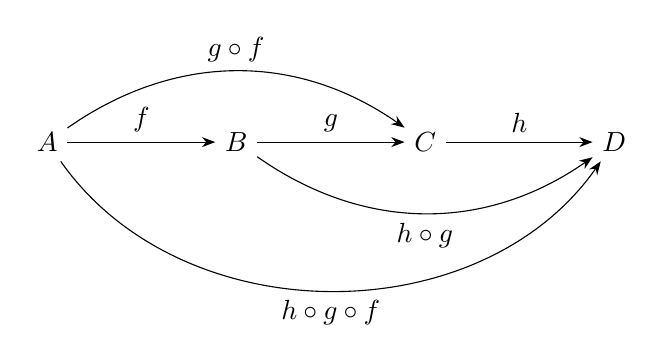
\begin{tikzpicture}[>=Stealth,node distance=2.4cm]
  \node (A) {$A$};
  \node (B) [right of=A] {$B$};
  \node (C) [right of=B] {$C$};
  \node (D) [right of=C] {$D$};
  \draw[->] (A) -- node[above]{$f$} (B);
  \draw[->] (B) -- node[above]{$g$} (C);
  \draw[->] (C) -- node[above]{$h$} (D);
  \draw[->,bend left=35] (A) to node[above]{$g\circ f$} (C);
  \draw[->,bend right=35] (B) to node[below]{$h\circ g$} (D);
  \draw[->,bend right=55] (A) to node[below]{$h\circ g\circ f$} (D);
\end{tikzpicture}
\end{center}

\subsection{Mono és epi: az injektivitás és a szürjektivitás \emph{nyíl}-nyelven}

A $\mathbf{Set}$ kategóriában a monomorfizmusok pontosan az injektív függvények
(\lean{Kategoria.mono\_iff\_inj}), az izomorfizmusok pontosan a bijekciók
(\lean{Kategoria.isIso\_iff\_bij}). Ezért a 2.18 feladat (,,injektívek
kompozíciója injektív'') \emph{nem} valós-analízis állítás: minden kategóriában igaz,
hogy monomorfizmusok kompozíciója monomorfizmus
(\lean{Kategoria.mono\_comp\_mono}), és ebből a $\mathbf{Set}$-beli eset
azonnal jön (\lean{Kategoria.inj\_comp\_of\_mono}).

\begin{center}
\begin{tikzpicture}[>=Stealth,node distance=2.6cm]
  \node (T) {$T$};
  \node (X) [right of=T] {$X$};
  \node (Y) [right of=X] {$Y$};
  \node (Z) [right of=Y] {$Z$};
  \draw[->,transform canvas={yshift=2.2pt}] (T) -- node[above]{$u$} (X);
  \draw[->,transform canvas={yshift=-2.2pt}] (T) -- node[below]{$v$} (X);
  \draw[->] (X) -- node[above]{$f$} (Y);
  \draw[->] (Y) -- node[above]{$g$} (Z);
\end{tikzpicture}
\end{center}
\noindent
Olvasat: ha $g\circ f\circ u = g\circ f\circ v$, akkor előbb $g$ monóságával
$f\circ u = f\circ v$, majd $f$ monóságával $u = v$. \emph{A kétszeri
,,balról egyszerűsítés'' a bizonyítás egésze} --- ez a papíron írt
,,tegyük fel, hogy $g(f(x_1)) = g(f(x_2))$'' érvelés nyíl-alakja.

\subsection{Involúció mint izomorfizmus: 2.7}

Az $f(x) = \frac{x+1}{x-1}$ függvény önmaga inverze az $\R\setminus\{1\}$ halmazon.
Ez Leanben nem csak egy azonosság (\lean{gyak\_2\_7\_involucio}), hanem egy
tényleges \emph{izomorfizmus-objektum}: \lean{Kategoria.gyak\_2\_7\_equiv} típusa
$\{x : \R \mid x \ne 1\} \simeq \{x : \R \mid x \ne 1\}$.
A tanulság: \emph{az inverz létezésének bizonyítása helyett érdemes az inverzet
adatként megadni}, mert akkor a további tulajdonságok számolással jönnek.

\begin{center}
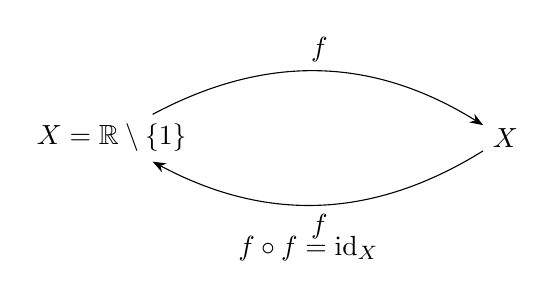
\begin{tikzpicture}[>=Stealth]
  \node (X) at (0,0) {$X = \R\setminus\{1\}$};
  \node (Y) at (5,0) {$X$};
  \draw[->,bend left=30] (X) to node[above]{$f$} (Y);
  \draw[->,bend left=30] (Y) to node[below]{$f$} (X);
  \node at (2.5,-1.4) {$f\circ f = \mathrm{id}_X$};
\end{tikzpicture}
\end{center}

\subsection{Univerzális tulajdonság: a szuprémum}

Az 1.4--1.5 feladatok magja: a szuprémum \emph{univerzális objektum}, ezért
egyértelmű (\lean{Kategoria.lub\_unique}, \lean{gyak\_1\_5}). A $(\R,\le)$ posetet
kategóriának tekintve $\sup S$ éppen az $S$ diagram \emph{kolimesze}: minden felső
korlát ,,alatta'' egy egyértelmű nyíllal.

\begin{center}
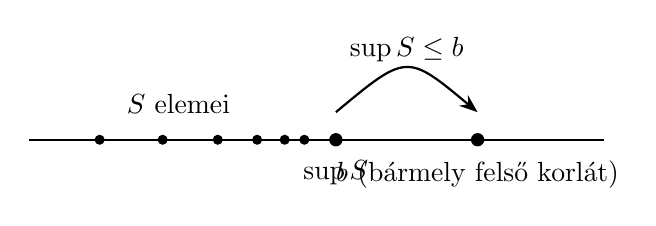
\begin{tikzpicture}[>=Stealth]
  \draw[thick] (-0.3,0) -- (7,0);
  \foreach \x/\lab in {0.6/,1.4/,2.1/,2.6/,2.95/,3.2/} \filldraw (\x,0) circle (1.6pt);
  \node at (1.6,0.45) {$S$ elemei};
  \filldraw (3.6,0) circle (2.2pt) node[below=4pt] {$\sup S$};
  \filldraw (5.4,0) circle (2.2pt) node[below=4pt] {$b$ (bármely felső korlát)};
  \draw[->,thick] (3.6,0.35) .. controls (4.5,1.1) .. (5.4,0.35);
  \node at (4.5,1.15) {$\sup S \le b$};
\end{tikzpicture}
\end{center}
\noindent
Következmény (a bizonyítási fogás): \emph{szuprémumot mindig két lépésben
igazolunk} --- (1) felső korlát, (2) minden felső korlátnál kisebb-egyenlő.
Leanben ez pontosan az \lean{IsLUB} definíciója, tehát a bizonyítás váza
\lean{constructor} $+$ két \lean{intro}.

\subsection{Galois-kapcsolat: az egészrész}

$\lfloor\cdot\rfloor : \R \to \Z$ a $\Z \hookrightarrow \R$ beágyazás
\emph{jobb adjungáltja}: $(z:\R) \le x \iff z \le \lfloor x\rfloor$
(\lean{Kategoria.floor\_galois}). A szokásos $x-1 < \lfloor x\rfloor \le x$
becslés (\lean{Kategoria.floor\_approx}) ennek puszta következménye.
Ugyanez a mintázat: $\sup$ balra adjungált a főideál-képzéshez
(\lean{Kategoria.sSup\_galois}).

\begin{center}
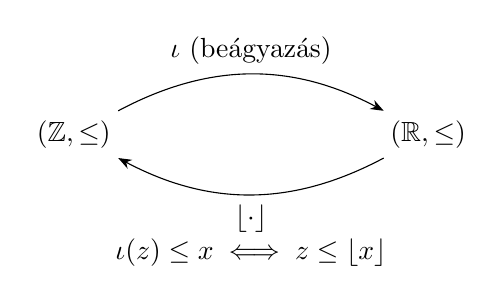
\begin{tikzpicture}[>=Stealth]
  \node (Z) at (0,0) {$(\Z,\le)$};
  \node (R) at (4.5,0) {$(\R,\le)$};
  \draw[->,bend left=28] (Z) to node[above]{$\iota$ (beágyazás)} (R);
  \draw[->,bend left=28] (R) to node[below]{$\lfloor\cdot\rfloor$} (Z);
  \node at (2.25,-1.5) {$\iota(z) \le x \iff z \le \lfloor x\rfloor$};
\end{tikzpicture}
\end{center}

\subsection{Szűrők: a határérték egyetlen fogalom}

Az egyetlen leghasznosabb strukturális belátás a 3.~feladatsorhoz: a
$\lim_{x\to a}$, $\lim_{x\to a^-}$, $\lim_{x\to\infty}$, $\to +\infty$
\emph{ugyanaz} a fogalom, csak más szűrővel. A projektben a
\lean{punktalt a := nhdsWithin a \{a\}ᶜ} rövidítés a ,,lyukas környezet'' szűrője.
A ,,határértékek behelyettesítési szabálya'' pedig egyszerűen
\emph{morfizmusok kompozíciója} (\lean{Kategoria.tendsto\_comp'}).

\begin{center}
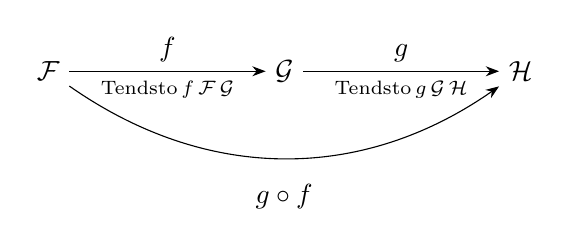
\begin{tikzpicture}[>=Stealth,node distance=3.0cm]
  \node (F) {$\mathcal{F}$};
  \node (G) [right of=F] {$\mathcal{G}$};
  \node (H) [right of=G] {$\mathcal{H}$};
  \draw[->] (F) -- node[above]{$f$} node[below]{\scriptsize$\mathrm{Tendsto}\,f\,\mathcal F\,\mathcal G$} (G);
  \draw[->] (G) -- node[above]{$g$} node[below]{\scriptsize$\mathrm{Tendsto}\,g\,\mathcal G\,\mathcal H$} (H);
  \draw[->,bend right=35] (F) to node[below=6pt]{$g\circ f$} (H);
\end{tikzpicture}
\end{center}

\noindent
Néhány szűrő és a hozzájuk tartozó ,,iskolás'' jelölés:
\begin{center}
\begin{tabular}{@{}lll@{}}
\toprule
Iskolás jelölés & Szűrő (Lean) & Példa \\
\midrule
$x\to a$ ($x\ne a$) & \lean{punktalt a} & \lean{gyak\_3\_1\_a} \\
$x\to a$ & \lean{nhds a} & \lean{gyak\_3\_13} \\
$x\to a^-$ & \lean{nhdsWithin a (Iio a)} & \lean{gyak\_3\_8\_b}, \lean{gyak\_3\_14} \\
$x\to 0^+$ & \lean{nhdsWithin 0 (Ioi 0)} & \lean{gyak\_4\_10\_q} \\
$x\to\infty$ & \lean{atTop} & \lean{gyak\_3\_2\_a}, \lean{gyak\_4\_10\_p} \\
$\to+\infty$ (cél) & \lean{atTop} & \lean{gyak\_3\_8\_e} \\
\bottomrule
\end{tabular}
\end{center}

\subsection{A láncszabály funktorialitása}

A legszebb kategóriaelméleti tartalom a 4.~feladatsorban van: a differenciálás
\emph{funktor}. A ,,pontozott sima leképezések'' kategóriájából a
lineáris leképezések kategóriájába megy, és megőrzi a kompozíciót és az identitást:
\[
  D(g\circ f)_x = D g_{f(x)} \circ Df_x, \qquad D(\mathrm{id})_x = \mathrm{id}.
\]
Ez Leanben \lean{Kategoria.fderiv\_functorial} és \lean{Kategoria.fderiv\_id'};
az egydimenziós, iskolás alak $\left(g(f(x))\right)' = g'(f(x))\,f'(x)$
(\lean{Kategoria.lancszabaly}, alkalmazva \lean{gyak\_4\_2\_lanc}-ban).

\begin{center}
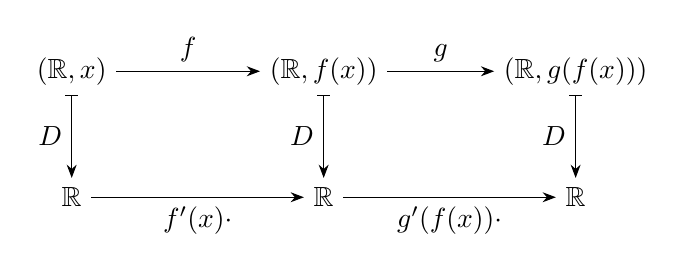
\begin{tikzpicture}[>=Stealth]
  \node (X) at (0,1.6) {$(\R,x)$};
  \node (Y) at (3.2,1.6) {$(\R,f(x))$};
  \node (Z) at (6.4,1.6) {$(\R,g(f(x)))$};
  \node (TX) at (0,0) {$\R$};
  \node (TY) at (3.2,0) {$\R$};
  \node (TZ) at (6.4,0) {$\R$};
  \draw[->] (X) -- node[above]{$f$} (Y);
  \draw[->] (Y) -- node[above]{$g$} (Z);
  \draw[->] (TX) -- node[below]{$f'(x)\cdot$} (TY);
  \draw[->] (TY) -- node[below]{$g'(f(x))\cdot$} (TZ);
  \draw[|->] (X) -- node[left]{$D$} (TX);
  \draw[|->] (Y) -- node[left]{$D$} (TY);
  \draw[|->] (Z) -- node[left]{$D$} (TZ);
\end{tikzpicture}
\end{center}
\noindent
Ceruzával: rajzolj két sort, felül a függvényeket, alul a deriváltjaikat, és
gondold végig, hogy \emph{a négyzet kommutál}. Ez a kép azonnal megmondja,
miért nem lehet a láncszabályban $f'$ és $g'$ argumentumát felcserélni.

\subsection{Monoton függvény mint funktor}

Egy rendezett halmaz kategória (egyetlen nyíl $x\to y$, ha $x\le y$), és egy
\emph{monoton} függvény pontosan egy funktor
(\lean{Kategoria.monotoneFunctor}); a funktorkompozíció pedig azt mondja,
hogy monoton függvények kompozíciója monoton (\lean{Kategoria.monotone\_comp}).
Ezért a 2.6 b) és 3.16 b) típusú monotonitási feladatok ugyanabba a keretbe esnek.

\section{Nagy ötletek (Big Ideas)}

\begin{bigidea}[Teljesség = a hiányzó pontok pótlása]
Az 1.~feladatsor minden ,,nemtriviális'' állítása a szuprémum-axiómán múlik:
$\sqrt2$ irracionális (1.9), a béka-sorozat (1.6) $1$-hez tart, de sosem éri el,
az $\{1/n\}$ halmaz infimuma $0 \notin \{1/n\}$ (1.4 c). Egy mondatban:
\emph{a $\Q$-ból $\R$-be lépés az, hogy a felülről korlátos halmazoknak
mostantól van legkisebb felső korlátjuk} --- és ez az egyetlen új dolog.
\end{bigidea}

\begin{bigidea}[Az egyenlőtlenség dinamikus, az egyenlőség statikus]
Indukciós egyenlőtlenségeknél (1.15) nem az állítást kell ,,látni'', hanem a
\emph{lépést}: mit kell hozzáadni a bal oldalhoz, és elég-e a jobb oldal
növekménye. Az 1.15 c)-ben az egész bizonyítás egyetlen lemma:
$\frac{1}{\sqrt{x+1}} < 2(\sqrt{x+1}-\sqrt x) < \frac1{\sqrt x}$
(\lean{sqrt\_lepes\_also}, \lean{sqrt\_lepes\_felso}).
\end{bigidea}

\begin{bigidea}[A határérték nem szám, hanem szűrő-morfizmus]
Ha ,,$x\to a$'' egy \emph{objektum} (szűrő), akkor a határérték-tételek
(összeg, szorzat, kompozíció, rendőrelv) mind ugyanannak a kategóriának a
szerkezeti tételei, és nem kell újratanulni őket a $x\to\infty$ esetre.
\end{bigidea}

\begin{bigidea}[Lokális linearizálás]
A derivált az a lineáris leképezés, amely $f$-et $x$ közelében a legjobban
közelíti. Ez a nézet magyarázza, miért funktor (4.2), miért igaz a L'Hospital-szabály
(4.10: két linearizálás hányadosa), és miért ,,romlik el'' $|x-2|$ a $2$-ben
(4.5 c: nincs \emph{egyetlen} legjobb lineáris közelítés, mert kétoldalt más).
\end{bigidea}

\begin{bigidea}[Kompaktság = a végtelen sok eset véges sokra redukálása]
A $[a,b]$-n folytonos függvény felveszi a maximumát; ezt használja a 4.9 és
--- meglepő módon --- a 4.13 is: a középpontosan konvex, folytonos függvény
konvexitását úgy kapjuk, hogy a hibafüggvény \emph{maximumhelyeinek} halmaza
zárt, tehát van legnagyobb eleme, és azt a középpont-egyenlőtlenséggel
,,jobbra toljuk''. Ez ellentmondás.
\end{bigidea}

\begin{bigidea}[Sűrűség + folytonosság = mindenütt]
Ha két folytonos függvény megegyezik egy sűrű halmazon, akkor egyenlő
(3.15). Ugyanez a mozdulat teszi lehetővé, hogy racionális (vagy diadikus)
pontokon dolgozzunk, és utána ,,átvigyük'' az állítást $\R$-re.
\end{bigidea}

\begin{bigidea}[Monoton + korlátos = konvergens]
A 3.14 és a 3.16 (az $e$ szám létezése) ugyanaz a séma: monotonitás $+$
korlátosság $\Rightarrow$ határérték. A határérték értékét \emph{nem}
kell ismerni --- ez az egzisztencia ereje.
\end{bigidea}

\begin{bigidea}[Univerzális tulajdonság $\Rightarrow$ egyértelműség ingyen]
Amit univerzális tulajdonsággal definiálunk (szuprémum, infimum, határérték,
inverz), az automatikusan egyértelmű. Az 1.5 feladat egy sablon, amelyet
mindenhol újra lehet használni.
\end{bigidea}

\section{Bizonyítási fogások, mozdulatok, rövidítések}

\subsection{Papíron és Leanben egyaránt működő mozdulatok}

\begingroup
\small
\begin{longtable}{@{}>{\raggedright\arraybackslash}p{3.2cm}>{\raggedright\arraybackslash}p{5.2cm}>{\raggedright\arraybackslash}p{6.4cm}@{}}
\toprule
\textbf{Mozdulat} & \textbf{Papíron} & \textbf{Leanben} \\
\midrule
\endfirsthead
\toprule
\textbf{Mozdulat} & \textbf{Papíron} & \textbf{Leanben} \\
\midrule
\endhead
\bottomrule
\endfoot
Definícióra bontás &
,,Azt kell megmutatni, hogy \dots'' &
\lean{constructor}, \lean{refine ⟨?\_, ?\_⟩}, \lean{intro} \\
Ekvivalencia két iránya &
,,$\Rightarrow$'', majd ,,$\Leftarrow$'' &
\lean{constructor} két ággal (\lean{gyak\_1\_12\_a}) \\
Esetszétválasztás &
,,$x \ge 0$ vagy $x < 0$'' &
\lean{rcases le\_or\_lt ..}, \lean{rcases abs\_cases ..} \\
Ellentmondás &
,,tegyük fel az ellenkezőjét'' &
\lean{by\_contra}, \lean{push\_neg} (\lean{gyak\_4\_13}) \\
Ellenpélda &
konkrét $x$ megadása &
\lean{refine ⟨fun x => .., ?\_⟩; norm\_num} (\lean{gyak\_2\_17\_a}) \\
Számolás &
,,rendezés után'' &
\lean{ring}, \lean{field\_simp}, \lean{nlinarith}, \lean{linarith} \\
Teleszkopizálás &
$\sum (a_{i+1}-a_i) = a_n - a_0$ &
\lean{Finset.sum\_range\_succ\_sub} / indukció \\
Becslés láncolása &
$A \le B \le C$ &
\lean{calc}, \lean{le\_trans}, \lean{linarith [..]} \\
,,Elég nagy $x$-re'' &
,,legyen $x > N$'' &
\lean{filter\_upwards [eventually\_gt\_atTop 0]} \\
Rendőrelv &
$|f| \le g \to 0$ &
\lean{squeeze\_zero\_norm'} és a rendőrelv-lemmák \\
Helyettesítés a határértékben &
$u = 3x$ &
kompozíció: \lean{Tendsto.comp} (\lean{gyak\_3\_7\_b}) \\
\end{longtable}
\endgroup

\subsection{Konkrét trükkök, amelyek a jelen formalizációt vitték}

\begin{trukk}[A meredekség-átírás: differenciahányadosból derivált]
A $\lim_{x\to0}\frac{\sin x}{x} = 1$, $\lim_{x\to 0}\frac{e^x-1}{x} = 1$,
$\lim_{x\to0}\frac{e^x-e^{-x}}{x} = 2$ típusú nevezetes határértékek
\emph{ugyanaz az állítás}, mint hogy a megfelelő függvény deriváltja $0$-ban
$1$, illetve $2$. Papíron ez a rövidítés az ,,ismerem a deriváltat, tehát
ismerem a határértéket'' irányba működik; Leanben az átírást a
\lean{hasDerivAt\_iff\_tendsto\_slope} lemma végzi
(\lean{gyak\_3\_7\_alap}, \lean{gyak\_4\_10\_f}).
\emph{Ez a legjobb ár-érték arányú fogás az egész 3--4. feladatsorban:}
egy nemtriviális határértékszámítást egy egysoros deriválásra cserél.
\end{trukk}

\begin{trukk}[Osztás a legmagasabb fokú taggal]
Racionális törtek $x\to\infty$ határértéke: oszd el a számlálót és a nevezőt
$x^k$-nal, majd használd, hogy $c/x^j \to 0$
(\lean{tendsto\_const\_div\_pow\_atTop}). Leanben az ,,osztás'' nem
átalakítás, hanem egy \emph{másik függvény}, amellyel a mienk
\emph{elég nagy} $x$-ekre megegyezik: ezért kell a
\lean{Filter.Tendsto.congr'} $+$ \lean{filter\_upwards} páros
(\lean{gyak\_3\_2\_a}).
\end{trukk}

\begin{trukk}[Gyöktelenítés]
$\sqrt{x^2+x}-\sqrt{x^2-x} = \dfrac{2x}{\sqrt{x^2+x}+\sqrt{x^2-x}}$: a
konjugálttal bővítés a $\infty-\infty$ határozatlan alakot $\frac{\infty}{\infty}$-re
cseréli, amit már az előző trükk kezel (\lean{gyak\_3\_3\_g}).
\end{trukk}

\begin{trukk}[Megszüntethető szakadás: szorzattá alakítás]
$\frac{t^2+3t-10}{t-2} = t+5$ (ha $t\ne2$). Leanben ez két lépés: a
$t\ne2$ helyeken a két függvény megegyezik (\lean{filter\_upwards
[self\_mem\_nhdsWithin]}), a $t+5$ pedig folytonos. A tanulság általános:
\emph{lyukas környezetben elég ,,majdnem mindenütt'' egyezés}
(\lean{gyak\_3\_12\_a}, \lean{gyak\_3\_12\_b}).
\end{trukk}

\begin{trukk}[Illesztés: folytonosság mint egyenlet a paraméterre]
A 3.13 és 4.7 feladatokban a ,,legyen folytonos/differenciálható'' feltétel
egy \emph{egyenletrendszer} a paraméterekre; a bizonyítás iránya
,,$\Leftarrow$'' konstrukció, ,,$\Rightarrow$'' pedig a féloldali határértékek
egyenlőségének kiolvasása. Leanben a darabonként definiált függvény
folytonosságát \lean{Continuous.if\_le} adja.
\end{trukk}

\begin{trukk}[Nem-differenciálhatóság: a féloldali meredekségek különböznek]
$|x-2|$ esetén nem kell semmit becsülni: ha differenciálható volna, a
differenciahányados határértéke egyszerre lenne $1$ és $-1$
(\lean{gyak\_4\_5\_c}). Az $x^{1/3}$ esetén a differenciahányados
$+\infty$-hez tart (\lean{gyak\_4\_5\_a}). \emph{Mindkettő ellentmondásos
bizonyítás, de a mag pozitív tartalom: kiszámoljuk a féloldali határértékeket.}
\end{trukk}

\begin{trukk}[Logaritmikus deriválás]
$x^x = e^{x\ln x}$: a hatványt exponenciálissá alakítva a láncszabály és a
szorzatszabály elvégzi a munkát (\lean{gyak\_4\_3\_xx}). Ugyanez az
átalakítás teszi értelmessé a $2^x$, $5^x$ deriváltjait is
(\lean{gyak\_4\_2\_szorzat}).
\end{trukk}

\begin{trukk}[Szélsőérték egyenlőtlenséggé alakítva]
,,$x e^x$ minimuma $-e^{-1}$'' helyett a formalizálható (és papíron is
tisztább) állítás: $\forall x,\; x e^x \ge -e^{-1}$
(\lean{gyak\_4\_8\_18\_min}). Ez a mozdulat --- \emph{szélsőérték-feladatból
egyenlőtlenség} --- a 4.11-ben is működik: $x(20-x)\le100$ egyetlen
\lean{nlinarith [sq\_nonneg (x-10)]} hívás, mert a bizonyítás lényege
a teljes négyzet $\big(x-10\big)^2 \ge 0$.
\end{trukk}

\begin{trukk}[A ,,legnagyobb maximumhely'' mozdulat (4.13)]
Ha $F$ folytonos $[0,1]$-en, $F(0),F(1)\le0$, és
$F\!\left(\frac{s+t}{2}\right)\le\frac{F(s)+F(t)}2$, akkor $F\le0$.
Bizonyítás: legyen $M = \max F$; ha $M>0$, akkor a
$S=\{t : F(t)=M\}$ halmaz zárt és korlátos, tehát $c=\sup S \in S$, és
$0<c<1$. Egy alkalmas $h>0$-ra
$M = F(c) \le \frac{F(c-h)+F(c+h)}2 \le \frac{M + F(c+h)}2$,
amiből $F(c+h)=M$, azaz $c+h\in S$ --- ellentmondás $c=\sup S$-sel.
\emph{Általános tanulság:} ha egy szélsőérték-hely nem egyértelmű, válaszd
a \emph{szélsőt} (a legnagyobbat), és told tovább.
\end{trukk}

\subsection{Lean-specifikus fogások (amelyeknek papíron is van tanulsága)}

\begin{itemize}
  \item \textbf{Először a váz.} Minden fájl úgy készült, hogy előbb a
    tételek \emph{kimondása} került be \lean{sorry}-val, és csak utána a
    bizonyítások. Papíron ugyanez: írd le pontosan, mit akarsz bizonyítani,
    mielőtt bizonyítanál --- a hibás kimondás a leggyakoribb időrabló.
  \item \textbf{Segédlemma-higiénia.} Az 1.15 c) és a 4.13 is akkor lett
    kezelhető, amikor a lényegi lépés önálló, névvel ellátott lemma lett
    (\lean{sqrt\_lepes\_also}, \lean{kozeppontos\_nonpos\_of\_endpoints}).
  \item \textbf{Az állítás ellenőrzése számpéldán.} Az 1.15 c) felső becslése
    $n=1$-re hamis; ez egyetlen behelyettesítéssel kiderül. Mindig próbálj
    ki két-három konkrét értéket, mielőtt bizonyítani kezdesz.
  \item \textbf{,,Majdnem mindenütt'' egyenlőség.} A \lean{Tendsto.congr'} és
    a \lean{filter\_upwards} formalizálja azt a papíros mondatot, hogy
    ,,elég nagy $x$-re'' vagy ,,$x\ne a$ esetén''.
  \item \textbf{Adat helyett tulajdonság, tulajdonság helyett adat.} Ha az
    inverz létezése kell, add meg az inverzet (\lean{Equiv}); ha csak az
    egyértelműség, elég az univerzális tulajdonság.
\end{itemize}

\section{Ceruzával rajzolható ábrák}

\subsection{Az $\varepsilon$--$\delta$ doboz (3.1)}

\begin{center}
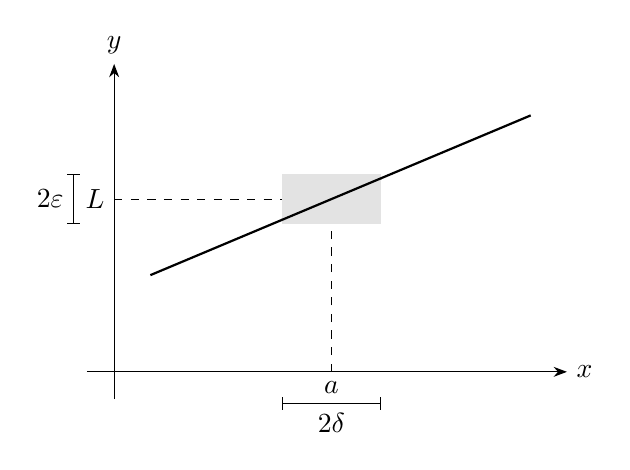
\begin{tikzpicture}[scale=1.15,>=Stealth]
  \draw[->] (-0.3,0) -- (5,0) node[right]{$x$};
  \draw[->] (0,-0.3) -- (0,3.4) node[above]{$y$};
  \draw[thick,domain=0.4:4.6,smooth,variable=\x] plot ({\x},{0.9+0.42*\x});
  \def\a{2.4} \def\L{1.908}
  \draw[dashed] (\a,0) -- (\a,\L);
  \draw[dashed] (0,\L) -- (\a,\L);
  \node[below] at (\a,0) {$a$};
  \node[left] at (0,\L) {$L$};
  \fill[gray!22] (\a-0.55,\L-0.28) rectangle (\a+0.55,\L+0.28);
  \draw[thick,domain=1.85:2.95,smooth,variable=\x] plot ({\x},{0.9+0.42*\x});
  \draw[|-|] (\a-0.55,-0.35) -- (\a+0.55,-0.35) node[midway,below]{$2\delta$};
  \draw[|-|] (-0.45,\L-0.28) -- (-0.45,\L+0.28) node[midway,left]{$2\varepsilon$};
\end{tikzpicture}
\end{center}
\noindent
\emph{Játék:} az $\varepsilon$-t a \emph{ellenfél} adja (magasság), a $\delta$-t
mi (szélesség). A rajz azt mutatja, hogy a $\delta$-széles függőleges sávban a
grafikon benne marad az $\varepsilon$-magas vízszintes sávban.

\subsection{Rendőrelv (3.3 i)}

\begin{center}
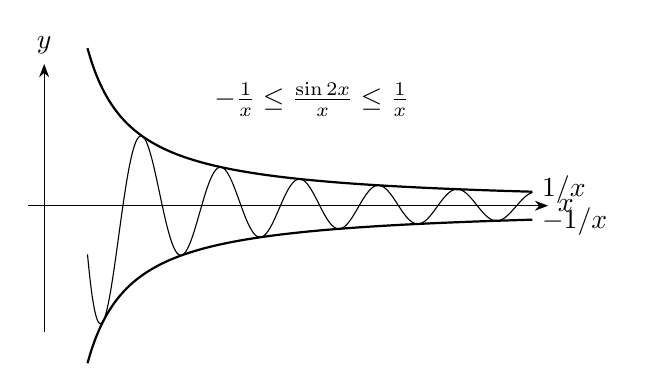
\begin{tikzpicture}[scale=1.0,>=Stealth]
  \draw[->] (-0.2,0) -- (6.4,0) node[right]{$x$};
  \draw[->] (0,-1.6) -- (0,1.8) node[above]{$y$};
  \draw[thick,domain=0.55:6.2,smooth,variable=\x,samples=120] plot ({\x},{1.1/\x});
  \draw[thick,domain=0.55:6.2,smooth,variable=\x,samples=120] plot ({\x},{-1.1/\x});
  \draw[domain=0.55:6.2,smooth,variable=\x,samples=250] plot ({\x},{1.1*sin(360*\x)/\x});
  \node[right] at (6.2,0.2) {$1/x$};
  \node[right] at (6.2,-0.2) {$-1/x$};
  \node at (3.4,1.35) {$-\tfrac1x \le \tfrac{\sin 2x}{x}\le \tfrac1x$};
\end{tikzpicture}
\end{center}

\subsection{Teleszkopikus becslés (1.15 c)}

\begin{center}
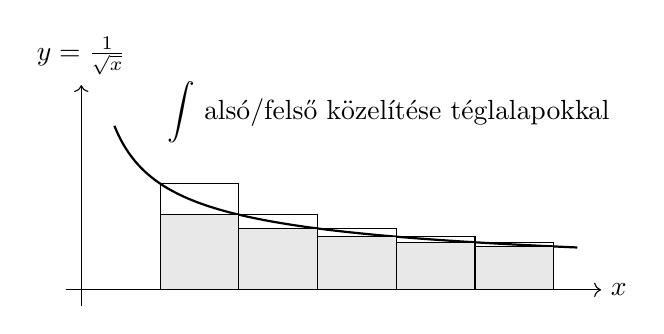
\begin{tikzpicture}[scale=1.0]
  \draw[->] (-0.2,0) -- (6.6,0) node[right]{$x$};
  \draw[->] (0,-0.2) -- (0,2.6) node[above]{$y=\frac{1}{\sqrt x}$};
  \draw[thick,domain=0.42:6.3,smooth,variable=\x,samples=200] plot ({\x},{1.35/sqrt(\x)});
  \foreach \i in {1,2,3,4,5}{
    \draw[fill=gray!18] (\i,0) rectangle (\i+1,{1.35/sqrt(\i+1)});
  }
  \foreach \i in {1,2,3,4,5}{
    \draw (\i,0) rectangle (\i+1,{1.35/sqrt(\i)});
  }
  \node at (3.9,2.25) {$\displaystyle\int$ alsó/felső közelítése téglalapokkal};
\end{tikzpicture}
\end{center}
\noindent
A $2(\sqrt{x+1}-\sqrt x)$ mennyiség éppen a görbe alatti terület egy lépésen;
ezt fogja közre a két téglalap: $\frac{1}{\sqrt{x+1}} < 2(\sqrt{x+1}-\sqrt x) < \frac1{\sqrt x}$.
Összegzésnél a jobb oldal ,,teleszkopál''.

\subsection{$(1+1/n)^n$: monoton és korlátos (3.16)}

\begin{center}
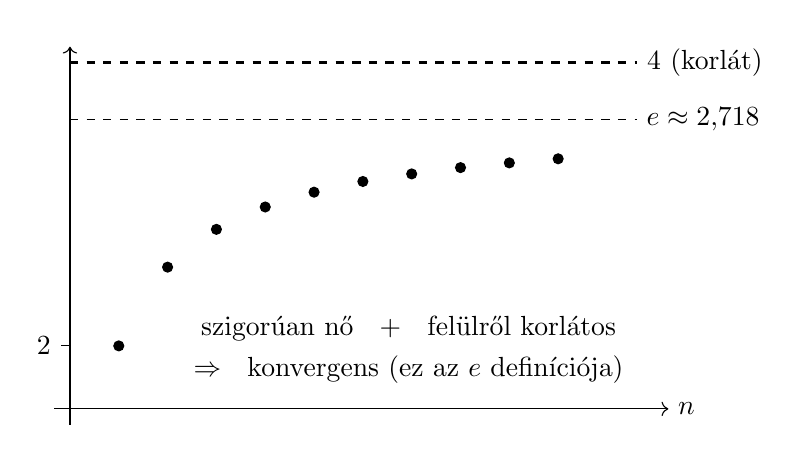
\begin{tikzpicture}[scale=1.0]
  \draw[->] (-0.2,0) -- (7.6,0) node[right]{$n$};
  \draw[->] (0,-0.2) -- (0,4.6) node[above]{};
  % y = (v - 1.8)*4
  \draw[dashed] (0,3.68) -- (7.2,3.68) node[right]{$e \approx 2{,}718$};
  \draw[dashed,thick] (0,4.4) -- (7.2,4.4) node[right]{$4$ (korlát)};
  \foreach \n/\v in {1/2.000,2/2.250,3/2.370,4/2.441,5/2.488,6/2.522,7/2.546,8/2.566,9/2.581,10/2.594}{
    \filldraw ({0.62*\n},{(\v-1.8)*4}) circle (1.8pt);
  }
  \draw (0,0.8) -- (-0.12,0.8) node[left]{$2$};
  \node[align=center] at (4.3,0.75) {szigorúan nő \; + \; felülről korlátos\\[1mm] $\Rightarrow$ \; konvergens (ez az $e$ definíciója)};
\end{tikzpicture}
\end{center}

\subsection{Középpontos konvexitás (4.13)}

\begin{center}
\begin{tikzpicture}[scale=1.25]
  \draw[->] (-0.2,0) -- (6.9,0) node[right]{$x$};
  \draw[->] (0,-0.2) -- (0,3.4) node[above]{$y$};
  \draw[thick,domain=0.4:5.6,smooth,variable=\x,samples=120] plot ({\x},{0.28*(\x-3)*(\x-3)+0.5});
  \def\p{1.1} \def\q{5.0}
  \filldraw ({\p},{0.28*(\p-3)*(\p-3)+0.5}) circle (1.4pt) node[left]{$(x,f(x))$};
  \filldraw ({\q},{0.28*(\q-3)*(\q-3)+0.5}) circle (1.4pt) node[right]{$(y,f(y))$};
  \draw[thick] ({\p},{0.28*(\p-3)*(\p-3)+0.5}) -- ({\q},{0.28*(\q-3)*(\q-3)+0.5});
  \def\m{3.05}
  \filldraw ({\m},{0.28*(\m-3)*(\m-3)+0.5}) circle (1.4pt);
  \filldraw ({\m},{0.5*(0.28*(\p-3)*(\p-3)+0.5)+0.5*(0.28*(\q-3)*(\q-3)+0.5)}) circle (1.4pt);
  \draw[<->,dashed] ({\m},{0.28*(\m-3)*(\m-3)+0.5}) -- ({\m},{0.5*(0.28*(\p-3)*(\p-3)+0.5)+0.5*(0.28*(\q-3)*(\q-3)+0.5)});
  \draw[dashed] ({\m},0) -- ({\m},{0.28*(\m-3)*(\m-3)+0.5});
  \node[below] at ({\m},0) {$\frac{x+y}{2}$};
\end{tikzpicture}
\end{center}
\[
  f\!\left(\tfrac{x+y}{2}\right) \;\le\; \tfrac{f(x)+f(y)}{2}
  \qquad\text{(a szaggatott függőleges szakasz a két oldal különbsége)}
\]

\subsection{Lagrange-féle középértéktétel: párhuzamos húr és érintő}

\begin{center}
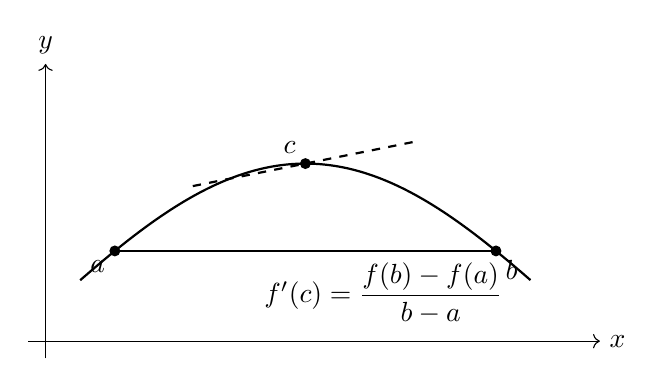
\begin{tikzpicture}[scale=1.1]
  \draw[->] (-0.2,0) -- (6.4,0) node[right]{$x$};
  \draw[->] (0,-0.2) -- (0,3.2) node[above]{$y$};
  \draw[thick,domain=0.4:5.6,smooth,variable=\x,samples=140] plot ({\x},{0.35+1.7*sin(30*\x)});
  \def\A{0.8} \def\B{5.2}
  \filldraw ({\A},{0.35+1.7*sin(30*\A)}) circle (1.6pt) node[below left]{$a$};
  \filldraw ({\B},{0.35+1.7*sin(30*\B)}) circle (1.6pt) node[below right]{$b$};
  \draw[thick] ({\A},{0.35+1.7*sin(30*\A)}) -- ({\B},{0.35+1.7*sin(30*\B)});
  \def\c{3.0}
  \draw[dashed,thick] ({\c-1.3},{0.35+1.7*sin(30*\c)-1.3*0.2}) -- ({\c+1.3},{0.35+1.7*sin(30*\c)+1.3*0.2});
  \filldraw ({\c},{0.35+1.7*sin(30*\c)}) circle (1.6pt) node[above left]{$c$};
  \node at (3.9,0.55) {$f'(c)=\dfrac{f(b)-f(a)}{b-a}$};
\end{tikzpicture}
\end{center}

\subsection{Inverz függvény: tükrözés az $y=x$ egyenesre (2.3, 2.6)}

\begin{center}
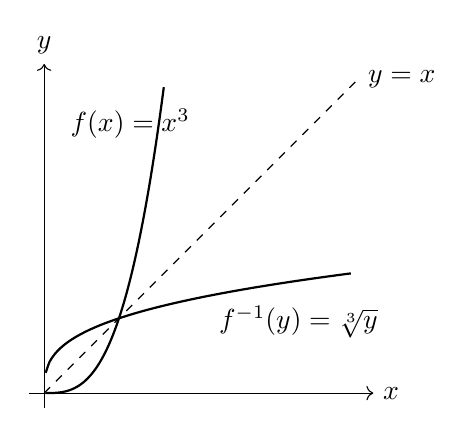
\begin{tikzpicture}[scale=0.95]
  \draw[->] (-0.2,0) -- (4.4,0) node[right]{$x$};
  \draw[->] (0,-0.2) -- (0,4.4) node[above]{$y$};
  \draw[dashed] (0,0) -- (4.2,4.2) node[right]{$y=x$};
  \draw[thick,domain=0.02:1.6,smooth,variable=\x,samples=80] plot ({\x},{\x*\x*\x});
  \draw[thick,domain=0.02:4.1,smooth,variable=\y,samples=80] plot ({\y},{pow(\y,0.3333)});
  \node at (1.15,3.6) {$f(x)=x^3$};
  \node at (3.4,0.95) {$f^{-1}(y)=\sqrt[3]{y}$};
\end{tikzpicture}
\end{center}
\noindent
Kategóriaelméleti olvasat: a tükrözés a $\mathbf{Set}$-beli izomorfizmus
,,fordított nyilát'' rajzolja ki.

\subsection{Nem differenciálható pontok (4.5)}

\begin{center}
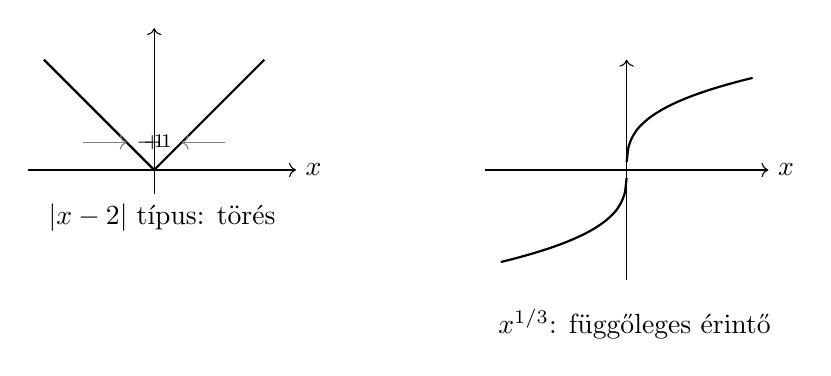
\begin{tikzpicture}[scale=1.0]
  \begin{scope}
    \draw[->] (-1.6,0) -- (1.8,0) node[right]{$x$};
    \draw[->] (0,-0.3) -- (0,1.8);
    \draw[thick] (-1.4,1.4) -- (0,0) -- (1.4,1.4);
    \node at (0.1,-0.6) {$|x-2|$ típus: törés};
    \draw[->,gray] (-0.9,0.35) -- (-0.35,0.35) node[right,black]{\scriptsize$-1$};
    \draw[->,gray] (0.9,0.35) -- (0.35,0.35) node[left,black]{\scriptsize$+1$};
  \end{scope}
  \begin{scope}[xshift=6cm]
    \draw[->] (-1.8,0) -- (1.8,0) node[right]{$x$};
    \draw[->] (0,-1.4) -- (0,1.4);
    \draw[thick,domain=0.001:1.6,smooth,variable=\x,samples=90] plot ({\x},{pow(\x,0.3333)});
    \draw[thick,domain=0.001:1.6,smooth,variable=\x,samples=90] plot ({-\x},{-pow(\x,0.3333)});
    \node at (0.1,-1.95) {$x^{1/3}$: függőleges érintő};
  \end{scope}
\end{tikzpicture}
\end{center}

\vspace{6mm}
\subsection{L'Hospital: két linearizálás hányadosa (4.10)}

\begin{center}
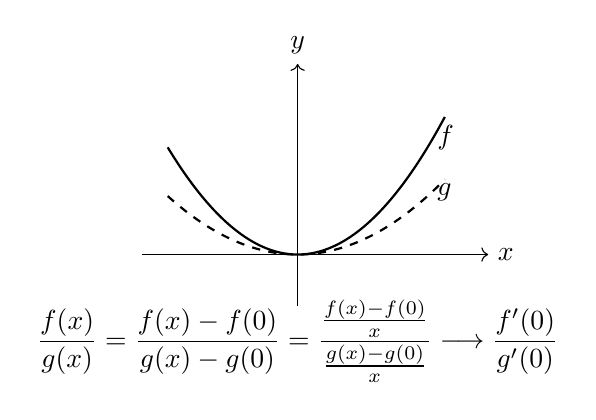
\begin{tikzpicture}[scale=1.1]
  \draw[->] (-1.8,0) -- (2.2,0) node[right]{$x$};
  \draw[->] (0,-0.6) -- (0,2.2) node[above]{$y$};
  \draw[thick,domain=-1.5:1.7,smooth,variable=\x,samples=100] plot ({\x},{0.55*\x*\x});
  \draw[thick,dashed,domain=-1.5:1.7,smooth,variable=\x,samples=100] plot ({\x},{0.30*\x*\x});
  \node[right] at (1.5,1.35) {$f$};
  \node[right] at (1.5,0.72) {$g$};
  \node at (0,-1.0) {$\dfrac{f(x)}{g(x)} = \dfrac{f(x)-f(0)}{g(x)-g(0)}
     = \dfrac{\frac{f(x)-f(0)}{x}}{\frac{g(x)-g(0)}{x}} \longrightarrow \dfrac{f'(0)}{g'(0)}$};
\end{tikzpicture}
\end{center}
\vspace{8mm}
\noindent
Ez a ,,kicsi'' L'Hospital: ha $f(0)=g(0)=0$ és $g'(0)\ne0$, akkor a hányados
határértéke a deriváltak hányadosa --- \emph{a differenciahányadossal való
bővítés az egész bizonyítás}. Ezt használja \lean{gyak\_4\_10\_f}, míg a
,,nagy'' L'Hospital (\lean{HasDerivAt.lhopital\_zero\_nhdsNE}) kell a
\lean{gyak\_4\_10\_e} esetben, ahol a nevező deriváltja is eltűnik.

\subsection{A szűrők ,,tölcsér'' képe}

\begin{center}
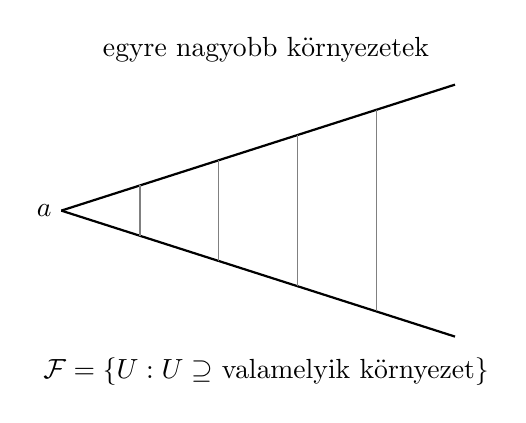
\begin{tikzpicture}[scale=1.0,>=Stealth]
  \draw[thick] (0,0) -- (5,1.6);
  \draw[thick] (0,0) -- (5,-1.6);
  \node[left] at (0,0) {$a$};
  \foreach \s in {1,2,3,4}{
    \draw[gray] ({\s},{-0.32*\s}) -- ({\s},{0.32*\s});
  }
  \node at (2.6,2.05) {egyre nagyobb környezetek};
  \node at (2.6,-2.05) {$\mathcal{F} = \{U : U \supseteq$ valamelyik környezet$\}$};
\end{tikzpicture}
\end{center}
\noindent
A szűrő nem más, mint annak a formalizálása, hogy ,,mit jelent közel lenni''.
Ha a $\mathcal F$ tölcsért a $f$ függvénnyel átvisszük, és a kép a
$\mathcal G$ tölcsérben marad, akkor $\mathrm{Tendsto}\ f\ \mathcal F\ \mathcal G$.
Innen a kompozíció-szabály nyilvánvaló: két tölcsért egymás után teszünk.

\section{Összefoglalás}

A gyakorlatok három szinten olvashatók:
\begin{enumerate}[nosep]
  \item \textbf{Technikai szint:} egy konkrét határérték, derivált, becslés.
  \item \textbf{Módszertani szint:} melyik fogást használjuk (gyöktelenítés,
        teleszkopizálás, meredekség-átírás, esetszétválasztás).
  \item \textbf{Strukturális szint:} melyik kategóriában dolgozunk, mi a
        funktor, mi az univerzális tulajdonság, mi az adjunkció.
\end{enumerate}
A formalizáció haszna éppen az, hogy a harmadik szintet láthatóvá teszi:
Leanben nem lehet ,,elhallgatni'' a szűrőt, a tartományt vagy a
differenciálhatóság feltételét, ezért a bizonyítás kénytelen a szerkezetet
megmutatni. Ugyanez a fegyelem papíron is működik --- és attól lesz egy
papíron írt bizonyítás rövid, hogy strukturálisan a helyes szinten van kimondva.

\end{document}
